\documentclass[12pt,a4paper]{article}
\usepackage{geometry}
\newgeometry{tmargin=2cm, bmargin=2cm, lmargin=2cm, rmargin=2cm}
\usepackage[T1]{fontenc}
\usepackage[polish]{babel}
\usepackage[utf8]{inputenc}
\usepackage{amsmath}
\usepackage{amssymb}
\usepackage{graphicx} % Usunięto [dvips] dla lepszej kompatybilności
\usepackage{listings}
\usepackage[usenames,dvipsnames]{xcolor}

\definecolor{mygreen}{RGB}{25,130,0}
\definecolor{mylilas}{RGB}{180,55,230}
\definecolor{myNumbers}{RGB}{180,222,230}

% Deklaracja brakującego znaku minusa, na wypadek gdybyś go nie zamienił ręcznie
\DeclareUnicodeCharacter{2212}{-}

\lstloadlanguages{Matlab}
\lstset{language=Matlab,
    breaklines=true,
    basicstyle=\ttfamily,
    columns=fullflexible,
    extendedchars=true,
    inputencoding=utf8,
    keepspaces=true,
    morekeywords={matlab2tikz},
    keywordstyle=\color{blue},
    identifierstyle=\color{black},
    stringstyle=\color{mylilas},
    commentstyle=\color{mygreen},
    showstringspaces=false,
    emph=[1]{if,while,for,end,break,function,return,error,disp,syms},
    emphstyle=[1]\color{red},
    tabsize=2,
    xleftmargin=2em,
    frame=single,
    framexleftmargin=1.5em,
    literate={ą}{{\k{a}}}1
           {ę}{{\k{e}}}1
           {ć}{{\'c}}1
           {ł}{{\l{}}}1
           {ń}{{\'n}}1
           {ó}{{\'o}}1
           {ś}{{\'s}}1
           {ź}{{\'z}}1
           {ż}{{\.z}}1
           {Ą}{{\k{A}}}1
           {Ę}{{\k{E}}}1
           {Ć}{{\'C}}1
           {Ł}{{\L{}}}1
           {Ń}{{\'N}}1
           {Ó}{{\'O}}1
           {Ś}{{\'S}}1
           {Ź}{{\'Z}}1
           {Ż}{{\.Z}}1,
}

\begin{document}

\section*{Zadanie 1}

Napisać funkcję, której argumentem jest dowolna funkcja symboliczna \textbf{f}. Funkcja ma wczytać liczbę \textbf{n} oraz sprawdzić, czy jest ona naturalna. Jeśli nie, ma powtórzyć wczytywanie do skutku. Następnie ma wygenerować na jednym wykresie wykresy wszystkich \textbf{n} pochodnych funkcji \textbf{f} w przedziale $\left[-2\pi, 2\pi\right]$. Sprawdzić działanie dla funkcji $f(x) = x^5$ oraz $n = 5$. Załączyć wykres.

\vspace{1em}

\begin{lstlisting}
% Funkcja generująca na jednym wykresie n pochodnych funkcji f w przedziale
% [-2pi, 2pi]. Argumentem funkcji musi być funkcja symboliczna oraz liczba
% n , którą wprowadzamy musi być liczbą naturalną , co jest sprawdzanie
% przez funkcje.

function rysuj_pochodne(f_sym)
    if ~isa(f_sym,'sym')
        error('Argument musi być wyrażeniem symbolicznym (sym).')
    end
    
    syms x;
    while true
        n = input("Podaj liczbę naturalną n: ");
        if isnumeric(n) && isscalar(n) && n > 0 && n == round(n)
            break;
        else
            disp("Błąd: Wprowadzona wartość nie jest liczbą naturalną. " + ...
                "Spróbuj ponownie.")
        end
    end

    figure;
    hold on;
    grid on;
    title(['Wykresy ', num2str(n), ' pierwszych pochodnych']);
    xlabel('x');
    ylabel('y');
    xlim([-2*pi, 2*pi])

    pochodna = f_sym;
    colory = lines(n);

    for i = 1:n
        pochodna = diff(pochodna, x);
        h = fplot(pochodna, [-2*pi, 2*pi]);
        set(h, 'color', colory(i,:),'linewidth',1.5,'DisplayName', ...
            ['Pochodna ',num2str(i), ' rzędu.'])
    end

    legend('show','location','best');
    hold off;

    print -depsc wykres_pochodne.eps
end
\end{lstlisting}

\begin{lstlisting}
% Wywołanie funkcji dla zadanych parametrów
syms x
f = x^5;
rysuj_pochodne(f)
\end{lstlisting}

\begin{figure}[h]
    \centering
    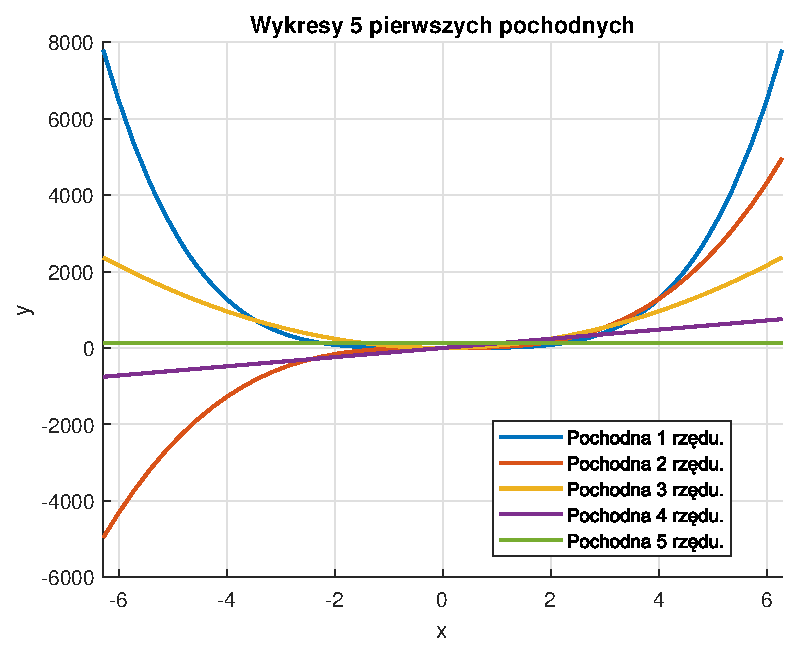
\includegraphics[width=0.8\textwidth]{wykres_pochodne.eps}
    \caption{
    Wykresy 5 pierwszych pochodnych funkcji $f(x)=x^5$
    }
    \label{fig:wykresy}
\end{figure}

\end{document}